% LaTeX Template for Project Report, Version 2.0
% (Abstracted from a Major Project Report at CSED, NIT Calicut but can be
% modified easily to use for other reports also.)
%
% Released under Creative Commons Attribution license (CC-BY)
% Info: http://creativecommons.org/licenses/by/3.0/
%
% Created by: Kartik Singhal
% BTech CSE Batch of 2009-13
% NIT Calicut
% Contact Info: kartiksinghal@gmail.com
%
% It is advisable to learn the basics of LaTeX before using this template.
% A good resource to start with is http://en.wikibooks.org/wiki/LaTeX/
%
% All template fields are marked with a pair of angular brackets e.g. <title here>
% except for the ones defining citation names in ref.tex.
%
% Empty space after chapter/section/subsection titles can be used to insert text.
%
% Just compile this file using pdflatex after making all required changes.

\documentclass[12pt,a4paper]{report}
\usepackage{textcomp}
\usepackage{tabulary}
\usepackage[pdftex]{graphicx} %for embedding images
\usepackage{url} %for proper url entries
\usepackage[bookmarks, colorlinks=false, pdfborder={0 0 0}, pdftitle={<pdf title here>}, pdfauthor={<author's name here>}, pdfsubject={<subject here>}, pdfkeywords={<keywords here>}]{hyperref} %for creating links in the pdf version and other additional pdf attributes, no effect on the printed document
%\usepackage[final]{pdfpages} %for embedding another pdf, remove if not required

\begin{document}
\renewcommand\bibname{References} %Renames "Bibliography" to "References" on ref page
\setlength{\parindent}{0pt}


%include other pages

\begin{titlepage}

\begin{center}

\textup{\bf Master Project Report} \\[0.2in]

% Title
\Large \textbf {Teakwood: An Web Framework for Handling Many-task Computing}\\[0.5in]

       \small \emph{Submitted in partial fulfillment of\\
        the requirements for the degree of}
        \vspace{.2in}

       {\bf Master in System Science} \\in\\Louisiana State University and Agricultural and Mechanical College\\ The School of Electrical Engineering and Computer Science\\
Computer Science and Engineering Division\\[0.5in]

% Submitted by
\normalsize by \\
\begin{table}[h]
\centering
\begin{tabular}{lr}\hline \\
Rui Guo \\ \\ \hline
 
%<Roll no here> & <Name here> \\
%<Roll no here> & <Name here> \\ 
%<Roll no here> & <Name here> \\ \\ \hline 
\end{tabular}
\end{table}

\vspace{.1in}
Under the guidance of\\
{\textbf{Jian Zhang}}\\[0.2in]

\vfill



%% Bottom of the page

\includegraphics[width=0.18\textwidth]{./nitc-logo}\\[0.1in]
%\Large{Department of Computer Science and Engineering}\\
%\normalsize
%\textsc{National Institute of Technology Calicut}\\
%Calicut, Kerala, India -- 673 601 \\
%\vspace{0.2cm}
\\
Fall Semester 2014

\end{center}
\end{titlepage}


\newpage
\thispagestyle{empty}
\mbox{}
%\begin{center}
\bf {Preface}\\[1.0cm]
\end{center}

Four years ago, I worked for an professor


\vspace{2in}

\begin{abstract}
Using Linux commands to handle computing jobs can be a hurdle to those scientific researchers who don't have HPC related background. Teakwood provides a solution and beyond. Teakwood is a framework that migrates all the terminal typing work to a web console GUI, and provides user a total control of their jobs, data, computing resources and so on simply by clicking functional buttons. Teakwood is also an open platform that enables user to work cooperatively. Through Teakwood, user can share their models, results, and computing resources within their group and have discussions in Teakwood forum. 
\end{abstract} 


\pagenumbering{roman} %numbering before main content starts
\tableofcontents
\listoffigures

\newpage
\pagenumbering{arabic} %reset numbering to normal for the main content

\chapter{Introduction}

\section{Motivation}
Four years ago, I know nothing about Linux. I then got a job to deal with HPC(High Cerformance Computing) system. Suddenly I jumped in to an UNIX environment. I found all those GUIs(Graphic User Interfaces), which I used to when I use Window OS, are gone, and I have to use Linux commands to control those machines and manage my stuff, which makes me uncomfortable and cumbersome. With the time goes by, I can work with Linux comfortably now. however, I still have the tendency to use GUI.\\I am not the only one that had such experience, In my working building, a lot of Scientists and researchers are suffering this pain. Further, cross-platform work adding them many wasteful jobs. For example, scientist A want to share a computing result for researcher B to do visualization. A uses Linux and B uses Window. What should they do? command, command, command, copy, paste, command, command ...\\Why not create a GUI platform to reduce those repeated typing work and allow them to work cooperatively?\\With all those desires, Here comes the Teakwood framework.

\section{Teakwood}
Teakwood is GUI framework that allows user to summit HPC jobs from its web console, and to have a full control of their job status. Teakwood also provides a file management systems for user to organize their job data easily. What's more, Teakwood enables user to work cooperatively by sharing their result, models and computing resources within their group. \\Teakwood migrates all the terminal typing work to Teakwood GUI, enables user to submit the HPC jobs just by simply clicking functional buttons.\\Teakwood is a web framwork, which means user can access from any type of machine as lons as the machine has a browser.

\section{Feature}
Functionally, Teakwood have the following features:\\
\\
$\bullet$ \textbf{Perfect documentation}\\
\\
Teakwood homepage provides diverse software information including installation guide, user manual, developer manual,video tutorial, etc. user can easily fetch info and grasp Teakwood soon.\\
\\
$\bullet$ \textbf{Extensible deployment}\\
\\
Teakwood is loose coupling designed. User can easily add or remove features, models or even python functions without mess the whole system.\\
\\
$\bullet$ \textbf{Neat GUI}\\
\\
A neat LSU style web console makes your work simple as Windows. Drag, push, click, that's it!\\
\\
$\bullet$ \textbf{Job monitor System}\\
\\
Job monitor system provides five labels: uploading, queued, running, finish, and Data ready to let the user monitor the job status. Job monitor system also periodically pulls the running message and displays it in the console, user can know more details about their job.\\
\\
$\bullet$ \textbf{Project management system}\\
\\
All user's project is well organized and web kept in a file server. user can compare, share, and download them as needed.\\
\\
$\bullet$ \textbf{Powerful admin}\\
\\
The powerful admin system is provided by Django itself. with tiny System configuration, use can activate their models.



 %literature survey included in this
\chapter{Teakwood System }

\section{Overview}
Structurally, like most websites, Teakwood system has a three layers layout: frontend, backend, and database. Becuase Teakwood will use computing servers to run jobs, so the eco Teakwood system actually has four layers, the up mentioned three plus the computing layer. the below figure shows how it looks like:\\

\begin{figure}[htb]
\centering
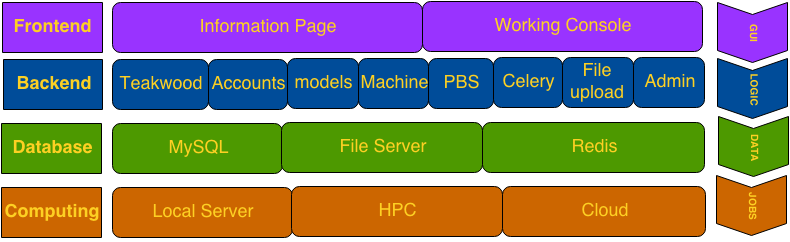
\includegraphics[scale=0.5]{./system_structure} 
% e.g. insert ./image for image.png in the working directory, adjust scale as necessary
\caption{Teakwood System Overview}
\label{fig:label} % insert suitable label, this is used to refer to a fig from within the text as shown above
\end{figure}

On the above figure, we can see four straight layers bottom up. In each layer, the left part is the layer name, the middle part is the layer content, and the right part is layer reality. Let's go through these layers one by one.

\section{Frontend}
The frontend is a visible GUI that user interact with. Basically all what we can see from the Teakwood website can be called "frontend".  For neat purpose, Teakwood separated the frontend into two parts: the \textbf{information page} and the \textbf{working console}. See below:

\begin{figure}[htb]
\centering
%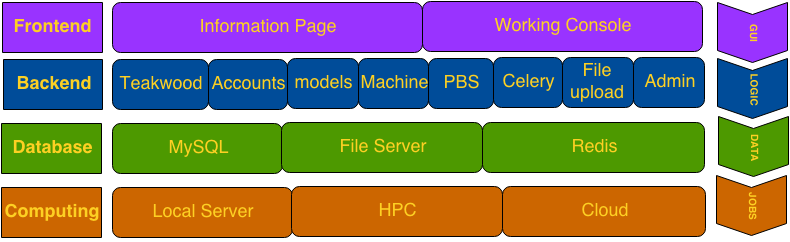
\includegraphics[scale=0.5]{./system_structure} 
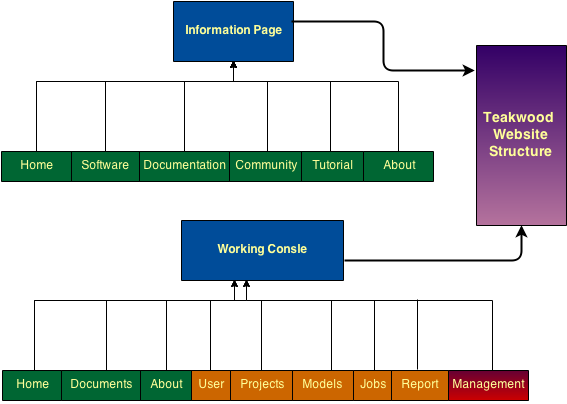
\includegraphics[scale=0.6]{./website_structure} % e.g. insert ./image for image.png in the working directory, adjust scale as necessary
\caption{Website Strucutre}
\label{fig:label} % insert suitable label, this is used to refer to a fig from within the text as shown above
\end{figure}

The \textbf{information page} introduces you all things about Teakwood.\\

$\bullet$ What is teakwood?\\
$\bullet$ What can Teakwood do?\\
$\bullet$ How to install Teakwood?\\
$\bullet$ How to use Teakwood?\\
$\bullet$ The user manual.\\
$\bullet$ Video tutorial.\\
$\bullet$ Teakwood forum.\\


The \textbf{working console} is your working place where you tango with your jobs and data. The functions buttons guide you to different places.\\

$\bullet$ \textbf{User}: Display user information.\\
$\bullet$ \textbf{Projects}: Create project and overview project.\\
$\bullet$ \textbf{Models}: Create model and overview model.\\
$\bullet$ \textbf{Jobs}:Create jobs, overview jobs and job monitoring.\\
$\bullet$ \textbf{Report}:Download job output.\\
$\bullet$ \textbf{Management}:Access to the admin system.\\


Note the color differences in the bottom layer.\\

$\bullet$ The \textbf{Green}: all visitors can see and manipulate.\\
$\bullet$ The \textbf{orange}: only logging user can see and manipulate.\\
$\bullet$ The \textbf{red}: only superuser can see and manipulate.\\


\section{Backend}
The backend is the logical design on how to interact with user. This Includes verifying user's request, pulling requested data, generating HTML web page and displaying web page. Teakwood follows the MVC(Model-View-Controller)design pattern and separates all the functions in to loose coupling parts, in Django, it call "app". All parts can both work independently and cooperatively.(We will have a backend chapter to reveal the logic mystery.)

In Teakwood system, there are mainly eight parts(Apps).\\

$\bullet$ \textbf{Teakwood}: control the frontend presentation.\\
$\bullet$ \textbf{Accounts}: control the user identification.\\
$\bullet$ \textbf{Models}: invoke and control the computing models.\\
$\bullet$ \textbf{machine}:invoke and control the computing resources\\
$\bullet$ \textbf{PBS}:Guide the PBS script generation.\\
$\bullet$ \textbf{File upload}:gather input files to buffer for downloading \\
$\bullet$ \textbf{Admin}:overall control of user and data.\\
$\bullet$ \textbf{Celery}:asynchronous handling.\\

\section{Data handling}
Teakwood system handles three types of data: the website data, the computing data and the message queue data. For each type of data we provide a different storage. see this table:\\
\\   
\begin{table}[h]
\begin{tabular}{lllll}
\cline{1-3}
\multicolumn{1}{|c|}{\textbf{Website data}} & \multicolumn{1}{c|}{\textbf{Computing data}} & \multicolumn{1}{c|}{\textbf{Message queue data}} &  &  \\ \cline{1-3}
\multicolumn{1}{|c|}{\textbf{MySQL}} & \multicolumn{1}{c|}{\textbf{File server}} & \multicolumn{1}{c|}{\textbf{redis server}} &  &  \\ \cline{1-3}
\multicolumn{1}{|c|}{\textbf{Teakwood data}} & \multicolumn{1}{c|}{\textbf{inputs and outputs}} & \multicolumn{1}{c|}{\textbf{Asynchronous handling}} &  &  \\ \cline{1-3}
                                &                                &                                &  & 
\end{tabular}
\end{table}


Teakwood website uses MySQL database for store it website data, e.g. the user account and the project labels.\\
For the computing data, we periodically rsync them to a separate file server for data  backup and downloading purpose. e.g. input files and the output result.\\
Message queue data is generated when we use Celery to asynchronous processing time consuming process. They are just ephemeral data, so we simply use a redis server to keep it.\\

\section{Remote Configuration}
Before the first time we can run a job in HPC or cloud, we have set up a connection and ready everything. the main things we should done are:\\

$\bullet$ Establish an password-less ssh log-in.\\
$\bullet$ Compile the tools and packages we will use in remote machine.\\
$\bullet$ Ready all the import path for Teakwood to use.\\

One those steps are done, we just simply "plug-in" Teakwood to the remote machine, and everything we can do from Teakwood web portal, without touch the under layers.


%\subsection{<Sub-section title>}

%\subsection{<Sub-section title>}
%some text\cite{citation-2-name-here}, some more text

%Refer figure \ref{fig:label}.



\chapter{Backend Mystery} 
Teakwood is powered by Django framework, so its backend inherits all the Django  backend feathers. For example, Teakwood follows the MVC(Model-View-Controller) design pattern and DRY(Don't Repeat Yourself) principle. When you go through Teakwood's code, you will find that teakwood have a neat and loose coupling coding structure. What makes Teakwood's coding structure so unique? This chapter will go through Teakwood's four important feathers in the backend: The MTV design pattern, the model to database mapping, the template language and the powerfull admin system.

\section{MTV Framework}
Teakwood has an updated MVC, that is MTV.\\
\begin{figure}[htb]
\centering
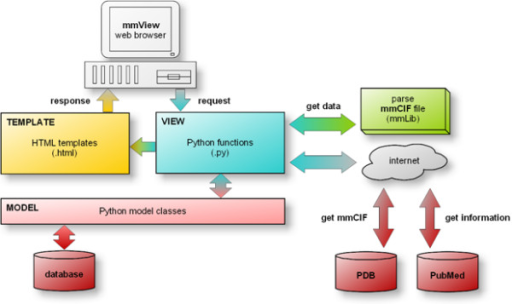
\includegraphics[scale=0.7]{./mtv}
\caption{Teakwood MTV framework}
\label{fig:label} % insert suitable label, this is used to refer to a fig from within the text as shown above
\end{figure}

\textbf{M} represents the model (Model), i.e., \textbf{the data access layer}. This layer processing data in all matters related to: how to access, how to confirm the validity , which behaviors it has, and the relationships between the data.\\
\textbf{T} Represents the template (Template), i.e., \textbf{the presentation layer}. This layer response for how to display the page or other types of documents.\\
\textbf{V} represents the view (View), \textbf{business logic layer}. You can see it as a bridge between the model and the template.This layer calls the model to provide data and sent it template for rendering web page. \\
\vspace{1in}

As we can see from the figure, Teakwood has a loose coupled modeling design. "M","T", and "V" are separated from each other; Each MTV wrapper(i.e. a Django app) is also separated from each other. This design makes the Teakwood sytem flexible for making changes and easy to extend feathers.

\section{Models and Database}
Teakwood provides an abstraction layer (the “models”) for structuring and manipulating the data of Teakwood apps. Essentially, a model is a Python object that describes your data model/table.Thanks for Django's integrated object relational mapping (ORM) functions, we don't have work with SQL database in order to manipulate data, all we should do is manipulating the corresponding Python object. ORM will do the mapping work.

Django provides many APIs to deal with Databases by invoking corespondent python object.

\section{Teakwood Template Language}
Teakwood’s template language is designed to strike a balance between power and ease. Its designed to please both the HTML designer and the Python coder. \\
Teakwood template language is not just HTML file or Python code. Here is an example:
\begin{verbatim}

{{ section.title }}

<h1>{{ section.title }}</h1>

<h2><a href="{{ story.get_absolute_url }}">
    {{ story.headline|upper }}
  </a></h2>
<p>{{ story.tease|truncatewords:"100" }}</p>


\end{verbatim}

We can see there are some special symbols in the HTML code. In Django template language they are called variables, tags and filters.\\

\textbf{Variable}: When the template engine encounters a variable, it evaluates that variable and replaces it with the result.\\
\textbf{Tag }: Tags are more complex than variables: Some create text in the output, some control flow by performing loops or logic, and some load external information into the template to be used by later variables. Some tags require beginning and ending tags. \\
\textbf{filter}:Filter is basically a restricted variable.\\

Through variables and tags, static HTML files becomes dynamic HTML files and can interact with python code. Django system even provides build-in tags for achieving the logical control.


\section{Powerful Admin}
Teakwood comes with a user authentication system which is inherited from Django framework also. The admin system handles user accounts, groups, permissions and cookie-based user sessions. 

Teakwood Admin system limited to trusted site administrators, that enables the adding, editing and deletion of site content. Some common examples: the interface you use to post to your blog, the backend site managers use to moderate user-generated comments, the tool your clients use to update the press releases on the Web site you built for them. All these cases can be handled in Admin console.

\section{A Practical Case}

So far we've already know that Teakwood is loose coupling designed and follows a "MTV"design pattern; we also know that Teakwood uses python object to work with database by object oriented mapping; plus, Teakwood template language is powerful for generating HTML files, now let's connect all these details to see How Teakwood process a request from user. 
Fisrt, let's take a look at the Teakwood HTTP request response flow.\\

\begin{figure}[h]
\centering
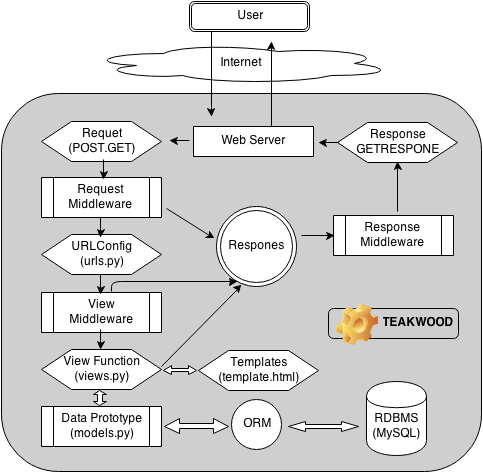
\includegraphics[scale=0.4]{./http_request_response}
\caption{Teakwood Request-Response Working Flow}
\label{fig:label} % insert suitable label, this is used to refer to a fig from within the text as shown above
\end{figure}
Now let take a real example to see how this structure works. For example, an user want to view all the job status under his/her account.
$\bullet$ Click the job button.\\
$\bullet$ Button triggered an request.\\
$\bullet$ Request goes to request middleware for identity check, if legal? auth?\\
$\bullet$ if yes, goes to response and raise error page;\\
$\bullet$ if no, goes to urlconfig to locate the right URL.\\
$\bullet$ URL goes to view middleware for legibility check, if wrong URL, auth?\\
$\bullet$ if yes, goes to response and raise an error page;\\
$\bullet$ if no, goes to view function. \\
$\bullet$ View function check if need data? if need template?\\
$\bullet$ if need data, trigger models to fetch data from database;\\
$\bullet$ if need template, find the right template, also fetch css, js and imgs.\\
$\bullet$ Send all files to response and rendering web page.\\
$\bullet$ Display the final page to user.



%\section{Lose Coupling}



\chapter{Asynchronous Handling} 

\section{Celery}
\section{RabbitMQ}
\chapter{Use Case} 

\section{Job Submission Flow}
\section{Job Monitoring}
\section{Job Report}
 
\chapter{Conclusion}

The primary goal of this report is to give the reader a general overview on Teakwood. The Deep inside Logic and the Database is hard to extend.

Teakwood is written in Python, so it will be good for scientific models to 
\chapter{Future Work}

\section{Docker Hub}
\section{Visualization}
\section{Computing on the GO}

\cleardoublepage
%\pagebreak
\phantomsection
\addcontentsline{toc}{chapter}{Acknowledgements}
\chapter*{Acknowledgments}
\vspace{1.0in}
Bootstrap CSS\\
Bootstrap JS\\
FAMFAMFAM icons\\
\newpage

\cleardoublepage
%\pagebreak
\phantomsection
\addcontentsline{toc}{chapter}{References}
\begin{thebibliography}{99}

\bibitem{citation-1-name-here}<Name of the reference here>,\ \url{<url here>}

\bibitem{citation-2-name-here}<Name of the reference here>,\ \url{<url here>}

\end{thebibliography}


\end{document}
